\section{Motivation}
\label{sec:motivation}

\ac{hci} studies the design of the interaction between computers and users. 
\citet{carlisle1976evaluating} was the first author who wondered about the 
interaction between humans and machines and several possible improvements. 
However, the term \ac{hci} was not used until 1980 
by~\citet{card1980keystroke}.

\ac{hci} is important because poorly designed human-machine interfaces can 
easily lead to unexpected problems. A classic example of this is the Three Mile 
Island accident, a nuclear meltdown accident, where the investigations concluded 
that the design of the human–machine interface was at least partially responsible 
for the disaster~\citep{nuclear2012backgrounder}. 

\begin{figure}[H]
\centering
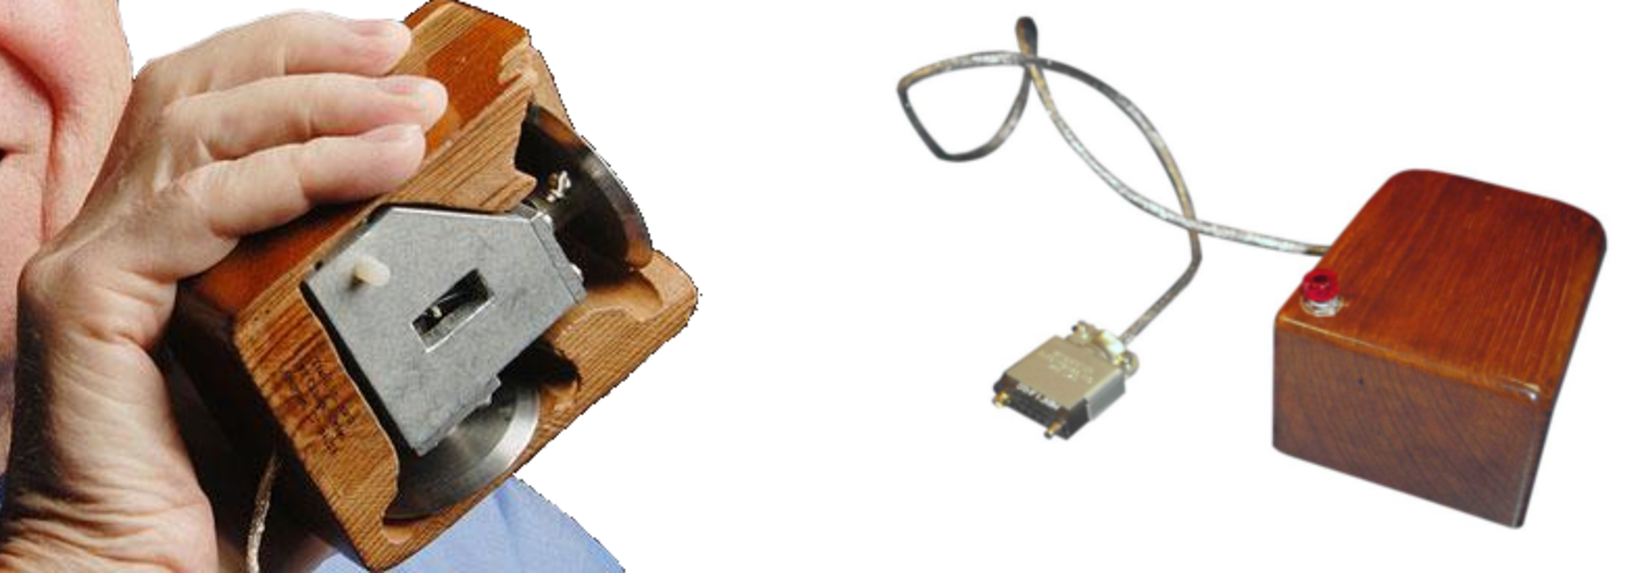
\includegraphics[width=0.70\textwidth]{mouse.pdf}
\caption{First computer mouse by Douglas Engelbart, formed by two wheels 
representing the two axis on the screen, and a single button.}
\label{fig:mouse}
\end{figure}

But the concept of \ac{hci} is not relegated to the past evolution of computers 
and industry. It has kept evolving and improving from the invention of the first
computer mouse (see Figure~\ref{fig:mouse}) by Douglas Engelbart during the 
sixties to nowadays interaction advances (see Figure~\ref{fig:google_glasses}).
This is thanks to emerging mobile and ubiquitous devices' capabilities, which
have opened new research domains and their power have outstripped the last
decades machines' computational capabilities. Besides, the \textit{mobile device}
concept is almost obsolete, since it has been replaced with what we know as
\textit{smartphones}. Smartphones are feature/mobile phones built over a mobile
operative system and more connectivity and computing capabilities. 

\begin{figure}[H]
\centering
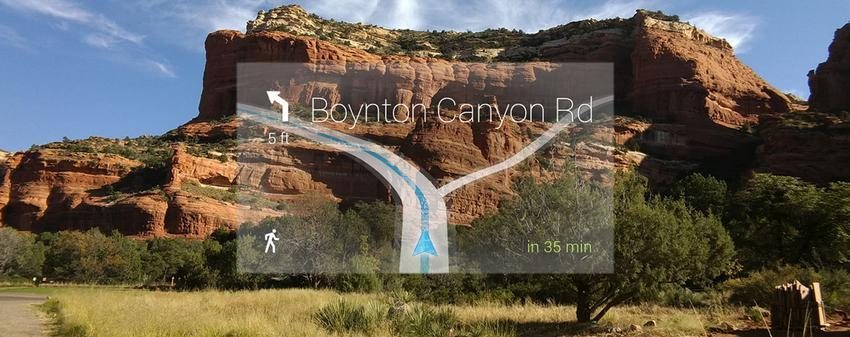
\includegraphics[width=0.70\textwidth]{google_glasses.jpg}
\caption{Google Glasses navigation interface~\citep{google_glasses}.}
\label{fig:google_glasses}
\end{figure}

Nevertheless, these devices are not just characterized by their power, process,
sensors and connectivity. They also allow developers and designers to include
customization and personalization features. Therefore, they are becoming more
than simple mobile phones. Now they are personal and intimate. They bring us
Internet, email, social networks (e.g., Facebook and Twitter) and so forth. They use
our habits and personal skills to recommend different resources, activities and
even people. And all of this just within reach.

But then, which is the motivation for this dissertation? The answer is found
regarding the target users of the cited adaptation approaches and advances.
To us developing for dependant users and users with disabilities is highly 
needed. Not significant efforts are currently being developed in this area, and 
how important might result having new tools for developers to make their 
applications inclusive. Besides, something that most systems regarding these 
users lack, is the consideration that users with similar disabilities might 
behave in different ways. This is due not only to their capabilities, but also 
due to the way they suffer them, or the influence of other capabilities. For 
example, blindness can be caused by several diseases, injuries, genetic defects 
or poisoning. In addition, people with the same disability might have different 
orientation perception, which might lead into different ways of suffering 
blindness.

Another reason which motivates this dissertation is the fact that nowadays the
share of people aged 65 represent a 17\% of the current European population. By
the year 2060 this figure is projected to rise to 30\%~\citep{european_comission_2012}.
As a consequence, and as the European Commission states, \textit{``the \ac{eu} 
would move from having four people of working-age to each person aged over 65 
years to about two people of working-age''}~\citep{european_comission_2012}.
The current situation shows that it is still a small group, but with a high 
expected increasing ratio. Nevertheless, this implies that we are still in time 
of accommodating, adapting and overtaking for future economic and demographic 
consequences.

Besides, systems personalization and environment components adaptation have been
demonstrated to benefit both users and service providers~\citep{kobsa_generic_2001}.
However, to achieve a satisfactory adaptation it is necessary to have several
inputs, for example, a user characteristics model. Hence, the service provider
will be able to apply the corresponding adaptations for the corresponding user.
In addition, current context conditions~\citep{jameson_modelling_2001} and user's
device capabilities are also crucial within this domain. 

On the other hand, being aware of what happens in the user's surroundings is what
researchers called context-awareness. Context-aware applications and systems have
been supported by the community for their significance within users focused
computing~\citep{schilit_context_aware_1994} \citep{chen_survey_2000}. It is
known that context affects user capabilities. In this dissertation we will see
how these capabilities are somehow influenced by context and how any adaptive
system should react to assure a minimum level of interaction with the user. As a
consequence, we will study each user, context and device capability and we will
present a model which allows to represent the interaction that these entities
may have. 

In spite of the research made by~\citet{kobsa_generic_2001}
and~\citet{fink_review_2000} to get generic user models (more focused on 
Artificial Intelligence) there is a lack of a common, exportable and standard 
models for these environments (adaptive user interface environments) (more 
details provided in Chapter~\ref{cha:state_of_the_art}). Most of the solutions 
presented in Chapter~\ref{cha:state_of_the_art} are strongly domain dependent. 
They rarely represent, for example, the influence of context variables in 
the current domain to perform adaptations. 

Therefore, there is a necessity of a solution for modelling every entity that
participates in an adaptive user interface environment and a methodology which
permits dynamic adaptations of these entities based on their mutually affecting
capabilities. This methodology will have to take into account several user
reactions with the adapted user interfaces. Consequently, an interaction model
for these environments will be required to evaluate user satisfaction with the
presented user interfaces


\subsection{User's context temporary disabilities}
\label{sec:context_disabilities}

\begin{description}
  \item[\Defi{Product design, by \citet{nelson1977home}}] \hfill \\
  \begin{mdframed}[hidealllines=true,backgroundcolor=gray!20]
  \textit{``Designing an object to be simple and clear takes at least twice as long as 
  the usual way. It requires concentration at the outset on how a clear and 
  simple system would work, followed by the steps required to make it come out 
  that way—steps which are often much harder and more complex than the ordinary 
  ones. It also requires relentless pursuit of that simplicity even when obstacles 
  appear which would seem to stand in the way of that simplicity.'' }
  \end{mdframed}
\end{description}  
  
This cite by \citeauthor{nelson1977home} introduced the problems that designing 
a product entails. One of the most significant issues to face during this process 
is the usability. According to the \acs{iso}/\acs{iec} 9126 standard~\citep{isoiec1}, 
quality represents a property of the software product defined in terms of a set 
of interdependent attributes (i.e., usability, security, reliability, performance, 
complexity, readability, reusability) expressed at different levels of detail 
and also taken into account the particular context of software use. At this 
point, the \acs{iso} 9241-11 standard states that usability is the extent to 
which a product can be used by specified users to achieve specified goals with 
effectiveness, efficiency and satisfaction in a specified context of 
use~\citep{iso9241}.

The interaction with devices needs to be satisfactory for the users. The 
\acs{iso}/\acs{iec} 9126-1~\citep{isoiec1} presents and details a two-part model 
for software product quality:

\begin{enumerate}
  \item Internal and external quality (see Figure~\ref{fig:ie_q_model}):
  Internal Quality is the totality of attributes of the software product from an
  internal view (e.g., spent resources, analysability). It is measured and
  improved during the code implementation, reviewing and testing. External 
  Quality is the quality when software is running in terms of its behaviour 
  (e.g., number of wrong expected reactions). It is measured and evaluated for 
  software testing in a simulated environment.
  
\begin{figure}[H]
\centering
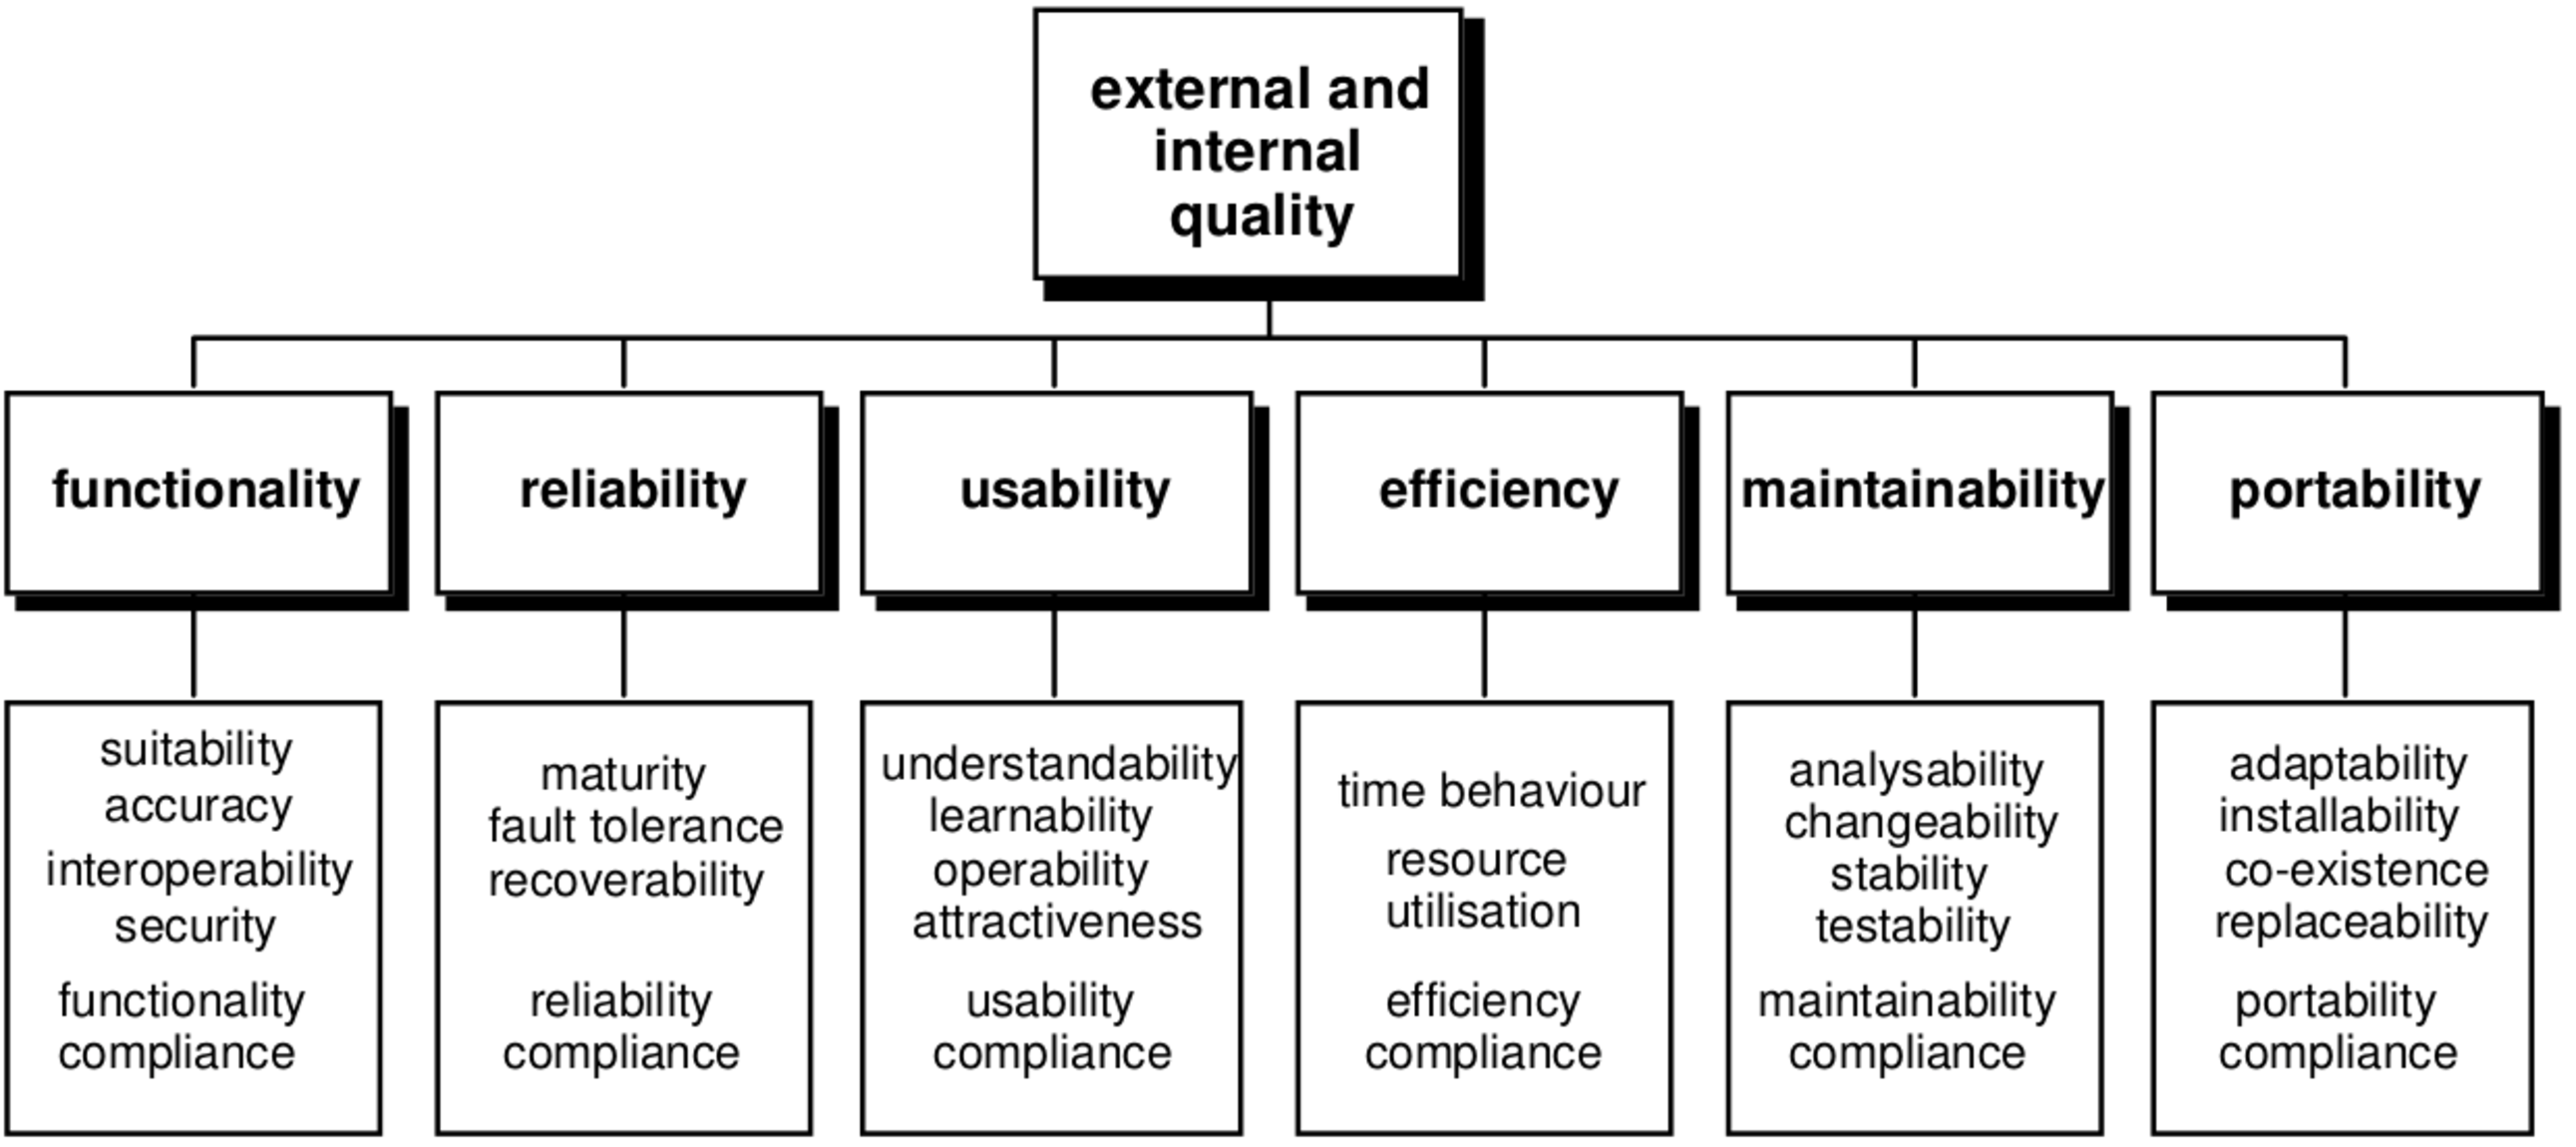
\includegraphics[width=0.75\textwidth]{internal_external_quality_model.pdf}
\caption{Quality model for external and internal quality~\citep{isoiec1}.}
\label{fig:ie_q_model}
\end{figure}
  
  \item Quality in use (see Figure~\ref{fig:qu_model}): It is the capability of
  the software product to enable specified users to achieve specified goals with
  effectiveness, productivity, safety and satisfaction in specified contexts of
  use.
\end{enumerate}


\begin{figure}[H]
\centering
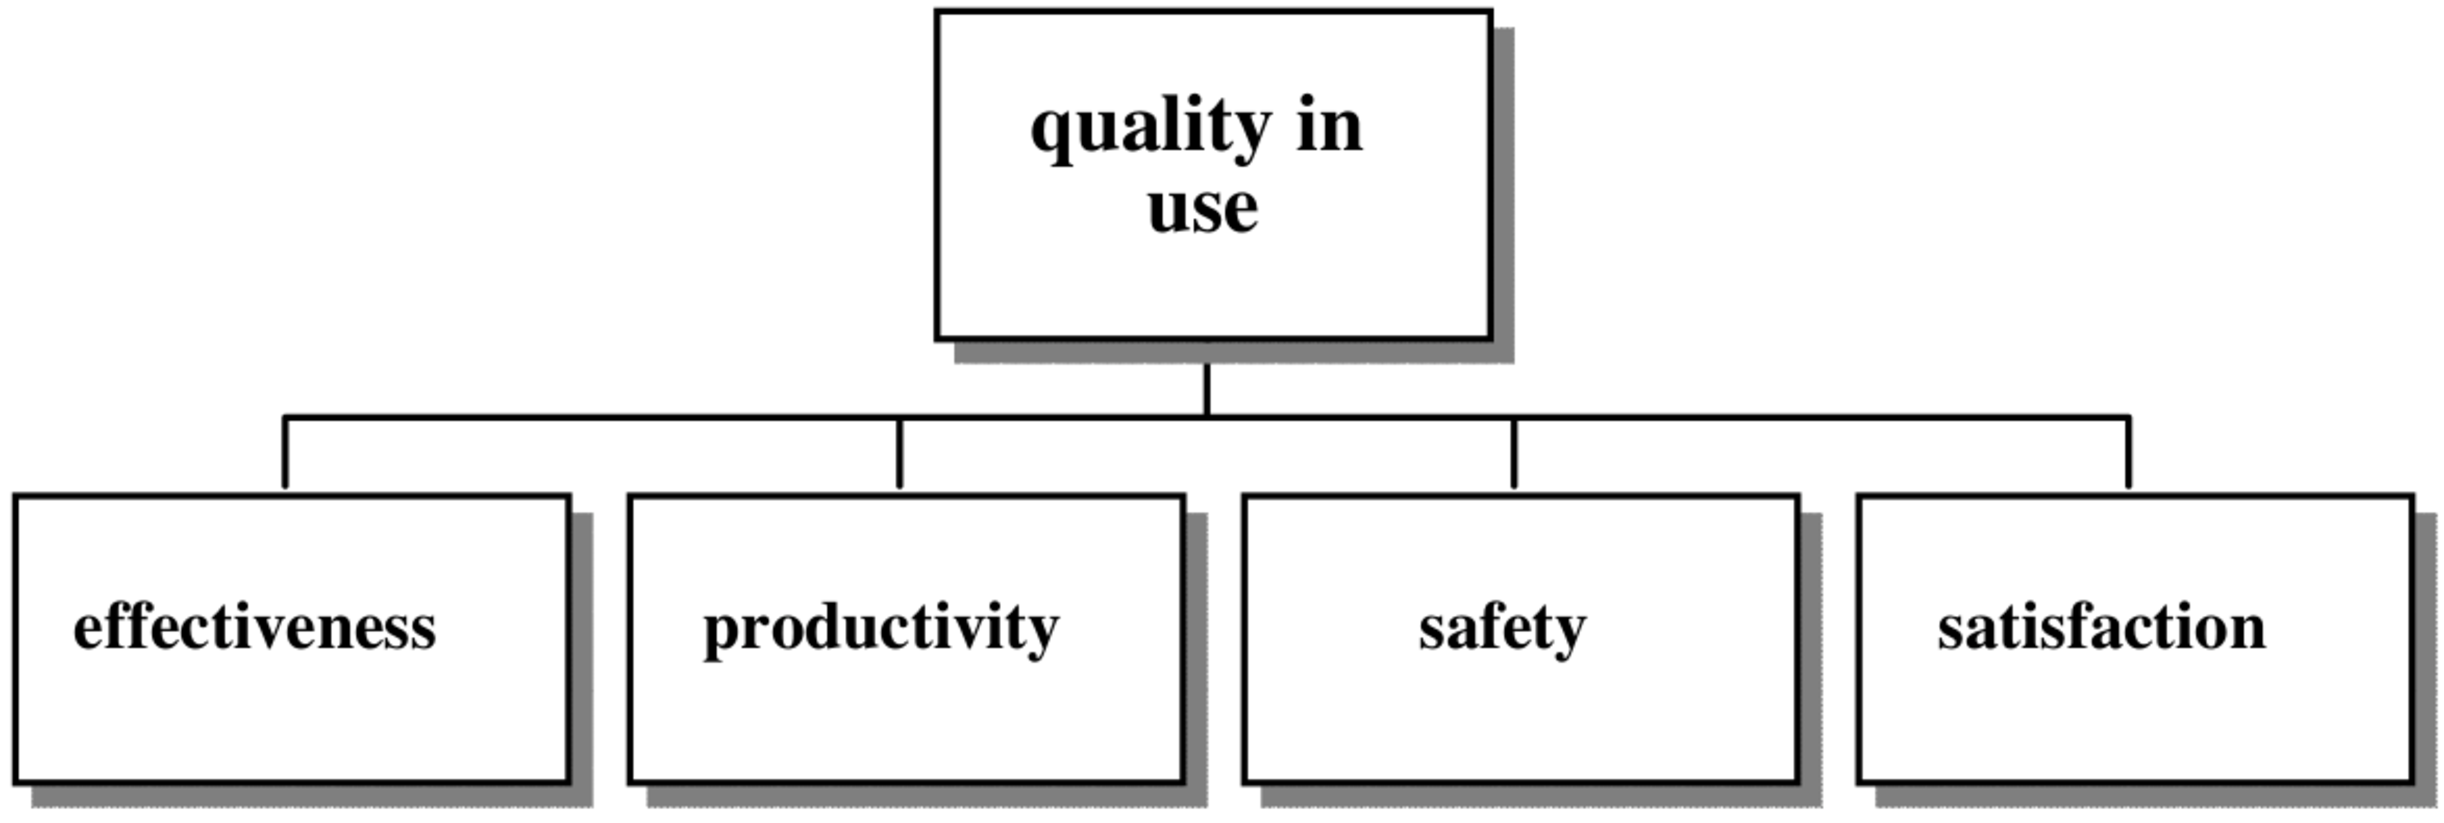
\includegraphics[width=0.5\textwidth]{quality_in_use_model.pdf}
\caption{Quality model for quality in use~\citep{isoiec1}.}
\label{fig:qu_model}
\end{figure}

However, the designing process becomes troublesome because of the nature of each
user. Users are very different from each others. They like different things and they
sense and perceive different. Moreover, they have different capabilities.
Besides, there are several groups which suffer these differences more deeply:
people with disabilities and the elderly. People with disabilities suffer from 
different impairments which are responsible for limiting several capabilities 
in a certain way. For example, users with sight disabilities will suffer from 
interaction problems with their devices if this interaction is based on visual 
stimulus (e.g., using a device display). On the other hand, elderly people 
usually suffer similar interaction troubles due to their ageing. As their 
senses tend to tire their capabilities and interaction levels decrease. Current 
technology trends try to reduce the interaction barriers that elderly suffer 
with nowadays devices. Mobile phones have audio control interaction and screen 
augmentation, \acsp{tv} have zoom and subtitles capabilities, and so on. 
Nevertheless, the elderly are used to use the products they already 
know~\citep{roupa_use_2010}~\citep{elderly_tech}.

% For these groups the designed devices should be [CITA]:
% 
% \begin{itemize}
%   \item \textit{Easy to use}, so the users are able to use them
%   to their own purposes.
%   \item \textit{``Easy to learn''}. This way, the final purpose of the
%   device should be affordable in an acceptable time interval.
%   \item \textit{Easy to recall}, so the users are able to remember how to interact
%   with the device.
% \end{itemize}

Nonetheless, people without disabilities are not exempt of suffering from very
similar situations. There are many conditions in which people without 
disabilities feel like if they had one. Using our smartphone when it is raining 
or with direct sunlight might affect our interaction with the device. These 
situations limit users' capabilities. They are examples of what context is and 
what it is capable of during an interaction process~\citep{dey_understanding_2001}. 
Desktop equipment are less prone to suffer from context conditions (obviously 
certain situations are impossible to avoid, like infrastructure problems). On 
the other hand, mobile devices are predisposed to experience problems due to 
current context situation. 
%[EXPLICAR O APUNTAR A OTRA SECCIÓN DONDE SE EXPLIQUE].

Context is essentially characterized by its capability of change. Besides, as it
is detailed in this dissertation context characteristics can affect several 
user's capabilities. Furthermore, it can change users' capabilities usually
reducing them as they have temporary disabilities. For example, direct sunlight
on a mobile phone screen reduce our sight capability; traffic or crowded streets
reduce our attention and hearing capabilities; several activities (e.g., driving
and cooking) and weather conditions (e.g., raining) affect our attention and
mobility. These are examples of \textit{user's context disabilities}. The first
approximation of this idea was conceived by reviewing the literature. More
specifically, and as it is shown in Chapter~\ref{cha:state_of_the_art}, the
thesis by~\citet{heckmann_ubiquitous_2005} presents the following illustration.

\begin{figure}[H]
\centering
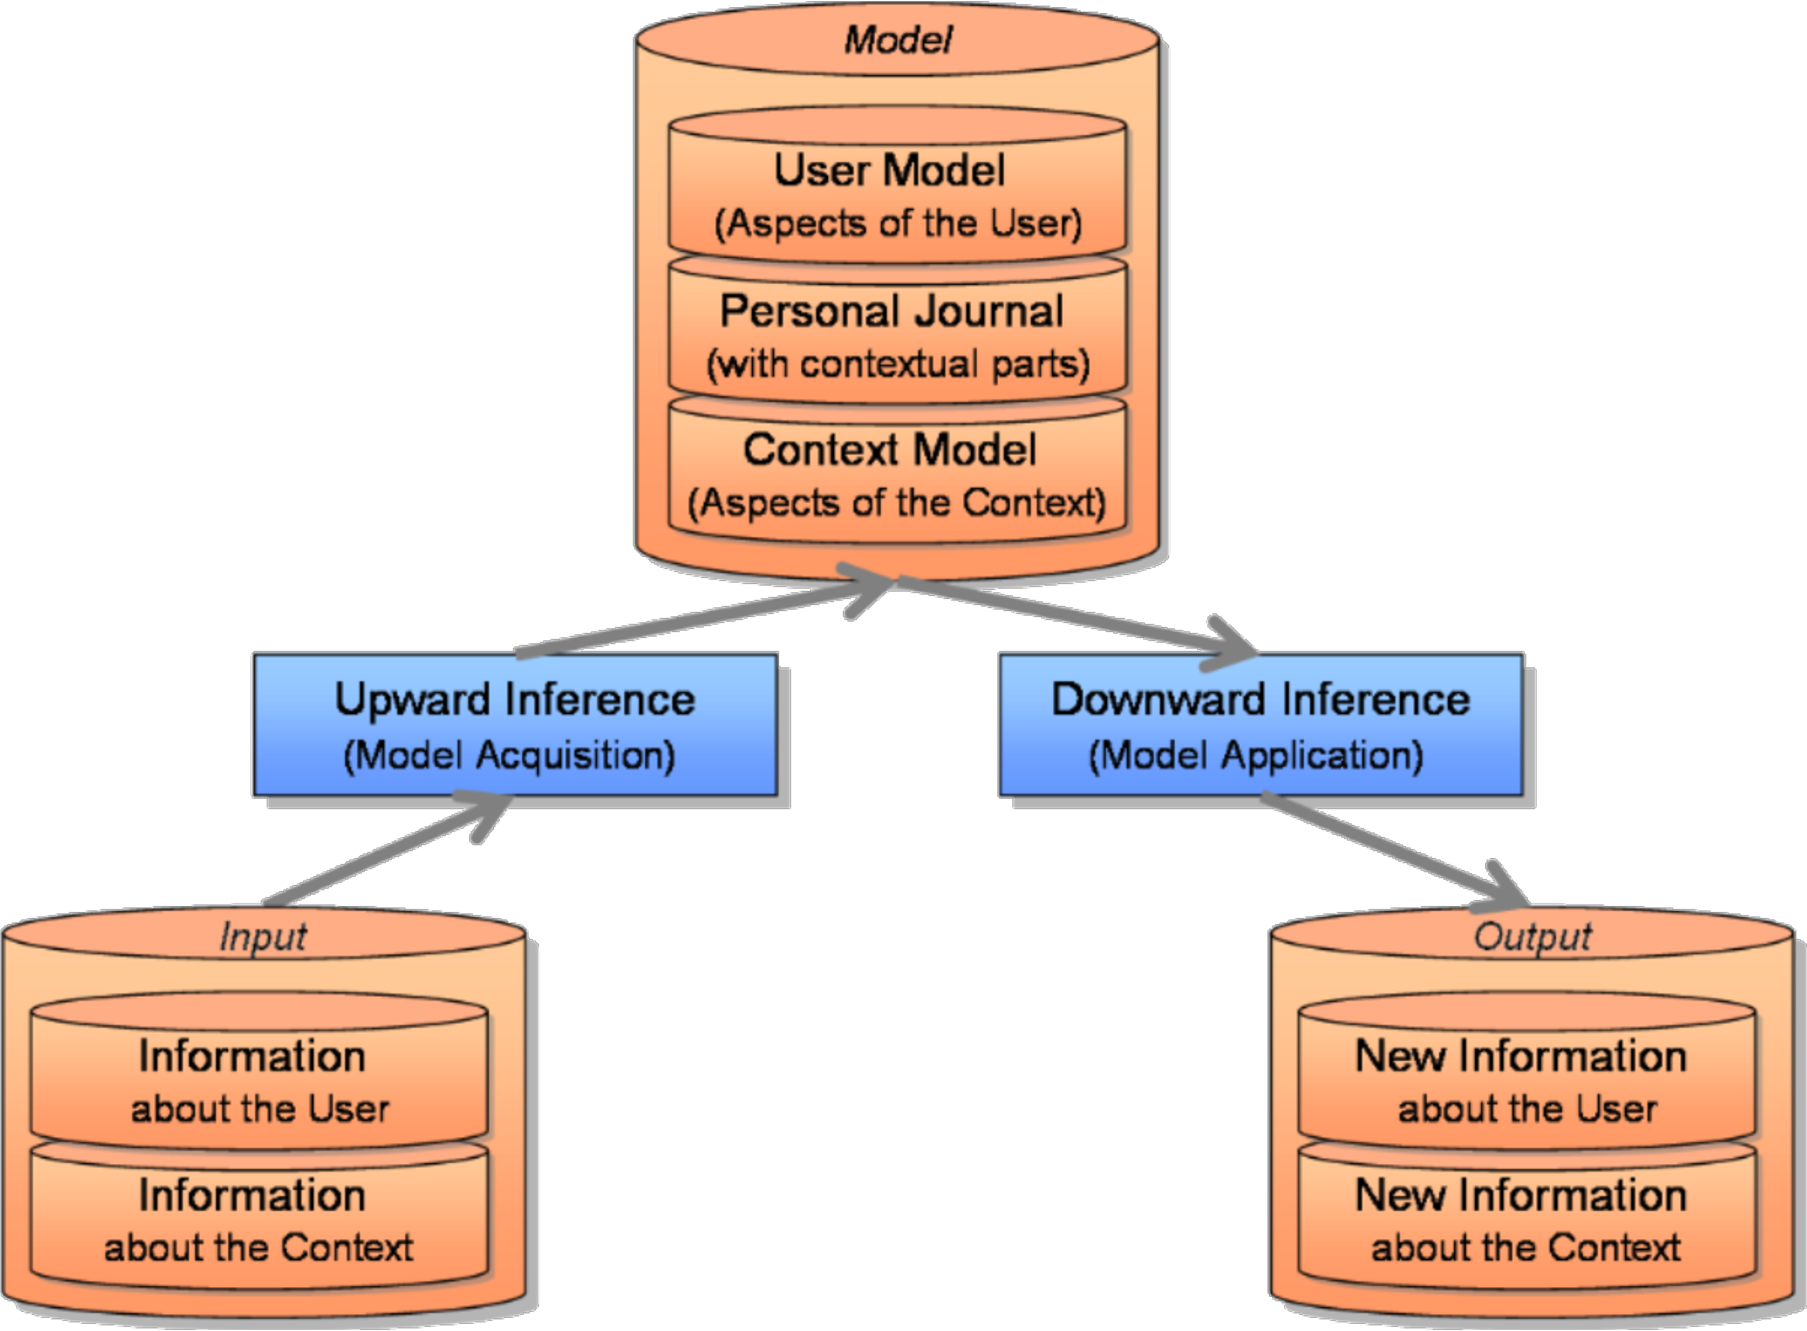
\includegraphics[width=0.6\textwidth]{heckmann.pdf}
\caption{Extended processing schema within context-aware user-adaptive systems, 
derived from~\citep{jameson_modelling_2001} and~\citep{kleinbauer_specter_user_centered_2003},
as appears in~\citep{heckmann_ubiquitous_2005}.}
\label{fig:heckmann}
\end{figure}

Figure~\ref{fig:heckmann} represents a conceptual view of the theory of user 
modelling with integrated context-awareness. In it there are a model acquisition
and model application information flows. From an \ac{ai} perspective, 
\citeauthor{heckmann_ubiquitous_2005} considers that the input data concerning 
the user and input data concerning the context are processed upward, as an 
inference step. This is what the author calls model acquisition. On the contrary,
the model application works downward, calculating a new hypothesis about the user
or the context. This idea made us understand the user, the context and the device
as evolutionary entities which, in each case, need from specific inference to
result into satisfactory usability with the user interface.

Hence, the main purpose of this dissertation is to dynamically reduce the 
disabilities caused by context on mobile devices by adapting their user interface. 
This will help to maintain certain levels of interaction with the users which 
would be impossible to reach in natural conditions.

\subsection{Definitions}
\label{sec:definitions}

In this section several significant definitions related to AdaptUI and user 
interface adaptation are given. Thus, the reading of the dissertation will be 
easier to understand.

\begin{description}
  \item[\Defi{User}] \hfill \\
  \begin{mdframed}[hidealllines=true,backgroundcolor=gray!20]
  As the main entity of the AdaptUI ecosystem, users are understood as individuals
  who have a set of interaction based characteristics. These characteristics might
  represent capabilities or even disabilities, but trough a semantic model which
  avoids the explicit representation of such concepts. 
  \end{mdframed}

  \item[\Defi{Context (I), by~\citet{dey_understanding_2001}}] \hfill \\
  \begin{mdframed}[hidealllines=true,backgroundcolor=gray!20]
  \textit{``Contex is any information that can be used to characterize the 
  situation of an entity. An entity is a person, place, or object that is 
  considered relevant to the interaction between a user and an application, 
  including the user and applications themselves''}. Context represents the 
  second main entity in the AdaptUI environment. In this dissertation we take
  this definition, as we believe it is the most popular definition regarding 
  the literature. As users and devices, context is semantically represented as 
  a set of characteristics which defines the current situation.
  \end{mdframed}
  
  \item[\Defi{Device}] \hfill \\
  \begin{mdframed}[hidealllines=true,backgroundcolor=gray!20]
  As the third entity in the AdaptUI ecosystem, devices represent the Android 
  based devices that users manipulate within the AdaptUI context. Devices are
  also understood as a series of characteristics which identify them, including
  both software and hardware related.
  \end{mdframed}
  
  \item[\Defi{Context-aware, by~\citet{schilit_disseminating_1994}}] \hfill \\
  \begin{mdframed}[hidealllines=true,backgroundcolor=gray!20]
  \textit{``Context-aware computing is the ability of mobile user's application 
  to discover and react to changes in the environment they are situated in.''} 
  In this dissertation several references to context-aware systems are made, 
  specially in Chapter~\ref{cha:state_of_the_art}.
  \end{mdframed}
  
  % \mydef{Environment}
  \item[\Defi{Adaptable user interface}] \hfill \\
  \begin{mdframed}[hidealllines=true,backgroundcolor=gray!20]
  In this dissertation we assume that adaptable user interfaces, as 
  as~\citet{fischer_user_2001} defines them, are those that change due to the 
  user intervention. In other words, not any user interface component adapts its
  shape or behaviour without the explicit user specification.
  \end{mdframed}

  \item[\Defi{Adaptive user interface}] \hfill \\
  \begin{mdframed}[hidealllines=true,backgroundcolor=gray!20]
  On the contrary, related to the previous definition, adaptive user interfaces
  have the ability to dynamically adapt themselves to the current task and user,
  not needing the user intervention~\citep{fischer_user_2001}. In the following
  chapters the reader will easily understand the differences between adaptable 
  and adaptive through several examples and the AdaptUI's architecture detail.
  \end{mdframed}

  \item[\Defi{User disability}] \hfill \\
  \begin{mdframed}[hidealllines=true,backgroundcolor=gray!20]
  This dissertation tries to reduce the possible (or temporary) disabilities 
  that the users might suffer when using their devices. To this end, a formal 
  definition of what a disability is is needed. As the \ac{icf} document defines, 
  disability \textit{``serves as an umbrella term for impairments, activity 
  limitations or participation restrictions.''}
  \end{mdframed}

  \item[\Defi{Context disabilities}] \hfill \\
  \begin{mdframed}[hidealllines=true,backgroundcolor=gray!20]
  AdaptUI focuses on the interaction of users suffering temporary disabilities 
  caused by the current context conditions. Thus, in this dissertation we 
  introduce the concept of context disabilities. To us, context disabilities 
  are basically temporary disabilities caused by the current context situation, 
  which might limit several user normal abilities or capabilities.
  \end{mdframed}

  \item[\Defi{Physiological capabilities}] \hfill \\
  \begin{mdframed}[hidealllines=true,backgroundcolor=gray!20]
  During the following chapters we refer to physiological capabilities as those 
  capabilities that are included in the \ac{icf} document under the sensory 
  functions classification.
  \end{mdframed}
 
  \item[\Defi{Ontology, by~\citet{gruber_translation_1993}}] \hfill \\
  \begin{mdframed}[hidealllines=true,backgroundcolor=gray!20]
  Ontologies are a \textit{``explicit specification of a conceptualization.''} 
  In other words, it is a formal mechanism to formally represents concepts of a 
  concrete domain.
  \end{mdframed}
  
  % \mydef{Semantics}
  \item[\Defi{Reasoning engine}] \hfill \\
  \begin{mdframed}[hidealllines=true,backgroundcolor=gray!20]
  A reasoning engine (or semantic engine) is a piece of software which is able 
  to infer logical consequences from a set of axioms or assertions. As defined
  in~\citep{owlapi_reasoners}, ``a reasoner is a key component for working with 
  \ac{owl} ontologies. In fact, virtually all querying of an \ac{owl} ontology 
  (and its imports closure) should be done using a reasoner. This is because 
  knowledge in an ontology might not be explicit and a reasoner is required to 
  deduce implicit knowledge so that the correct query results are obtained.''
  \end{mdframed}

  % Inclusive design is defined as follows~\citep{design_2005}: 
  \item[\Defi{Inclusive design}] \hfill \\
  \begin{mdframed}[hidealllines=true,backgroundcolor=gray!20]
  The design of mainstream products and/or services that are accessible to, and
  usable by, people with the widest range of abilities within the widest range
  of situations without the need for special adaptation or design~\citep{design_2005}.
  \end{mdframed}
\end{description}